%BOVY:NOTES:
% - We/I distinction
\documentclass[12pt,preprint]{aastex}
%\documentclass{emulateapj}
\usepackage{amssymb,amsmath}
%\usepackage{caption}
%\DeclareCaptionLabelSeparator{dotemdash}{.--- }
%\captionsetup[figure]{labelformat=simple, labelsep=dotemdash}
%\usepackage{color,hyperref}
% hypertex insanity
%\definecolor{linkcolor}{rgb}{0,0,0.25}
%\hypersetup{
%  colorlinks=true,        % false: boxed links; true: colored links
%  linkcolor=linkcolor,    % color of internal links
%  citecolor=linkcolor,    % color of links to bibliography
%  filecolor=linkcolor,    % color of file links
%  urlcolor=linkcolor      % color of external links
%}
\newcounter{address}
\setcounter{address}{1}
%\usepackage{sidecap}
\setlength{\emergencystretch}{2em}%No overflowing references
\newcommand{\ie}{i.e.}
\newcommand{\etal}{et al.}
\newcommand{\dd}{\mathrm{d}}
\newcommand{\eg}{e.g.}
\newcommand{\eqnname}{equation}
\newcommand{\Eqnname}{Equation}
\newcommand{\equationname}{\eqnname}
\renewcommand{\tablename}{Table}
\renewcommand{\figurename}{Figure}
\newcommand{\figurenames}{\figurename~s}
\newcommand{\sectionname}{$\mathsection$}
\newcommand{\normal}{\ensuremath{\mathcal{N}}}
\newcommand{\flag}[1]{\texttt{\lowercase{#1}}}
\newcommand{\feh}{\ensuremath{[\mathrm{Fe/H}]}}
\newcommand{\afe}{\ensuremath{[\alpha\mathrm{/Fe}]}}
\newcommand{\logg}{log g}
\newcommand{\Ro}{\ensuremath{R_0}}

\renewcommand{\vec}[1]{\ensuremath{\mathbf{#1}}}
\newcommand{\unitvec}[1]{\ensuremath{\mathbf{\hat{#1}}}}
\newcommand{\vecx}{\ensuremath{\vec{x}}}
\newcommand{\vecv}{\ensuremath{\vec{v}}}
\newcommand{\vech}{\ensuremath{\vec{H}}}
\newcommand{\vecj}{\ensuremath{\vec{J}}}
\newcommand{\vecp}{\ensuremath{\vec{p}}}
\newcommand{\vecn}{\ensuremath{\vec{n}}}
\newcommand{\veco}{\ensuremath{\vec{\Omega}}}
\newcommand{\veca}{\ensuremath{\boldsymbol\theta}}
\newcommand{\df}{\ensuremath{f}}
\newcommand{\tdf}{\ensuremath{\mathrm{tDF}}}
\newcommand{\paramsdiff}{\ensuremath{\vec{p}_\Delta}}
\newcommand{\paramsdf}{\ensuremath{\vec{p}_{\mathrm{DF}}}}
\newcommand{\paramspot}{\ensuremath{\vec{p}_\Phi}}
\newcommand{\sigv}{\ensuremath{\sigma_v}}

\newcommand{\DF}{\df}
\newcommand{\dff}{\ensuremath{\mathbf{f}}}
\newcommand{\dex}{\ensuremath{\,\mathrm{dex}}}
\newcommand{\Myr}{\ensuremath{\,\mathrm{Myr}}}
\newcommand{\Gyr}{\ensuremath{\,\mathrm{Gyr}}}
\newcommand{\kpc}{\ensuremath{\,\mathrm{kpc}}}
\newcommand{\pc}{\ensuremath{\,\mathrm{pc}}}
\newcommand{\kms}{\ensuremath{\,\mathrm{km\ s}^{-1}}}
\newcommand{\msun}{\ensuremath{\,\mathrm{M}_{\odot}}}
\newcommand{\inv}{\ensuremath{^{-1}}}

\newcommand{\jr}{\ensuremath{J_R}}
\newcommand{\jphi}{\ensuremath{J_\phi}}
\newcommand{\jz}{\ensuremath{J_Z}}
\newcommand{\lz}{\ensuremath{L_Z}}
\newcommand{\Or}{\ensuremath{\Omega_R}}
\newcommand{\Ophi}{\ensuremath{\Omega_\phi}}
\newcommand{\Oz}{\ensuremath{\Omega_Z}}
\newcommand{\ar}{\ensuremath{\theta_R}}
\newcommand{\aphi}{\ensuremath{\theta_\phi}}
\newcommand{\az}{\ensuremath{\theta_Z}}
\newcommand{\apar}{\ensuremath{\theta_\parallel}}
\newcommand{\opar}{\ensuremath{\Omega_\parallel}}
\newcommand{\aperp}{\ensuremath{\veca_\perp}}
\newcommand{\aperpii}{\ensuremath{\theta_{\perp,ii}}}
\newcommand{\operp}{\ensuremath{\veco_\perp}}
\newcommand{\operpii}{\ensuremath{\Omega_{\perp,ii}}}
\newcommand{\ts}{\ensuremath{t_s}}

\newcommand{\vlos}{\ensuremath{V_{\mathrm{los}}}}
\newcommand{\pmll}{\ensuremath{\mu_l}}
\newcommand{\pmbb}{\ensuremath{\mu_b}}

%\submitted{}

\begin{document}

\title{Dynamical modeling of tidal streams}
\author{Jo~Bovy\altaffilmark{\ref{Hubble}}}
\affil{Institute for Advanced Study, Einstein Drive, Princeton, NJ 08540, USA}
\email{bovy@ias.edu}
\altaffiltext{\theaddress}{\label{Hubble}\stepcounter{address} Hubble fellow}

\begin{abstract} 
  I present a new framework for modeling the dynamics of cold tidal
  streams. The framework consists of simple models for the initial
  action--angle distribution of tidal debris, which can be
  straightforwardly evolved forward in time. Taking advantage of the
  essentially one-dimensional nature of cold tidal streams, the
  transformation to position--velocity coordinates can be linearized
  and interpolated near a small number of points along the progenitor
  orbit, thus allowing for efficient computations of a stream's
  properties in observable quantities. I illustrate how to calculate
  the stream's average location (its ``track'') in different
  coordinate systems, how to quickly estimate the dispersion around
  its track, and how to draw mock stream data. As a generative model,
  this framework allows one to compute the full probability
  distribution function and marginalize over or condition it on
  certain phase--space dimensions as well as convolve it with
  observational uncertainties. This will be instrumental in proper
  data analysis of stream data. In addition to providing a
  computationally-efficient practical tool for modeling the dynamics
  of tidal streams, the action--angle nature of the framework helps
  elucidate in exactly what manner streams do not follow single
  orbits, how the observed width of the stream relates to the velocity
  dispersion or mass of the progenitor, and how the progenitors of
  ``orphan'' streams could be located.

  The practical usefulness of the proposed framework crucially depends
  on the ability to calculate action--angle variables for any orbit in
  any gravitational potential. A novel method for calculating actions,
  frequencies, and angles in any static potential using a single orbit
  integration is described in an Appendix.
\end{abstract}

\keywords{
        dark matter
        ---
	Galaxy: halo
	---
        Galaxy: kinematics and dynamics
        ---
	Galaxy: structure
        ---
        galaxies: interactions
        ---
        stellar dynamics
}


\section{Introduction}

Tidal streams hold enormous promise as probes of both the large-scale
structure of the Milky Way (MW) halo's density distribution
\citep[\eg,][]{Johnston99a,Koposov10a} and its small-scale
fluctuations \citep{Carlberg12a}. However, two factors
have hampered the practical use of tidal streams in obtaining
constraints on the MW gravitational potential. First, streams do not
trace a single orbit, which has led to confusion over how to best fit
streams and over how problematic the single-orbit approximation really
is \citep{Eyre11a,Sanders13a}. Second, approaches that go beyond the
single-orbit assumption encounter practical difficulties of
computational cost and observational data quality making many of these
approaches impractical for real, noisy data
\citep{Sanders13b,PriceWhelan13a}. Observed gaps in tidal streams may
be due to interactions with dark--matter subhalos \citep{Yoon11a}, but
spurious underdensities could be created by the dynamics of stream
stars. This hinders our ability to use underdensities in star counts
along a tidal stream in order to constrain the number of encounters
with dark satellites and their masses \citep{Ngan14a}. Fast,
generative models of tidal streams would greatly benefit both of these
applications.

It has long been clear that the dynamics of tidal streams is most
simply described in terms of action--angle coordinates
\citep{Tremaine99a,Helmi99a}. Once a star has been tidally stripped
from the progenitor, the self-gravity of the stream can be neglected
and the orbital actions of a stream member are conserved while the
angles increase linearly with time. The action--angle structure of a
stream is therefore characterized by strong but straightforward
correlations between the actions and angles of stream members, the
exploitation of which is crucial for using streams to measure the host
gravitational potential \citep{Sanders13b}. The description of a
stream in action--angle coordinates also elucidates the connection
between the orbit and velocity dispersion (or mass) of the progenitor
and the action distribution of the tidal debris \citep{Eyre11a},
allowing simple physical models of the stream to be used and to be
constrained by observational data.

However, streams are observed in position--velocity coordinates and
for action--angle descriptions to be useful, we must be able to
calculate the transformation between these coordinate systems
efficiently. Until now this has required accurate phase--space data
and specialized algorithms to calculate action--angle coordinates that
break down for the eccentric orbits on which tidal-stream progenitors
are typically found (that is, radial and/or vertical actions of
similar size as the angular momentum; \citealt{Sanders12a}). However,
even with Gaia, future stream data will typically have large
uncertainties compared to the intrinsic dispersion of the stream and
in particular the line-of-sight velocities of the faintest stream
members will not be observed for many stars. Additionally, streams are
superimposed on a non-negligible background of field stars and
background contamination cannot be easily taken into account in any of
the current stream-fitting methods.

In this paper, I present a new method for modeling cold tidal streams
that fundamentally lives in frequency--angle space, because the stream
distribution function is essentially one-dimensional in this
space. While many of the results of this paper are more generally
valid, the fiducial stream model in this paper consists of a
three-dimensional (close to) Gaussian distribution of frequencies in
the stream, a three-dimensional Gaussian distribution of initial angle
offsets between stream members and the progenitor, and a uniform
distribution of stripping times; the frequency and angle distributions
are independent of stripping time. While this model oversimplifies the
real stripping process, it is argued that at least for constraining
the gravitational potential with stream data, this simple model is
likely unbiased. For detailed mock stream data, more elaborate models
of the stripping process as a function of time might be necessary and
I discuss how these could easily be incorporated into the proposed
framework.

To evaluate the model in position--velocity coordinates, the
transformation to and from action--angle coordinates is computed using
a novel method for calculating action--angle coordinates presented in
Appendix~\ref{sec:aa}. This transformation is linearized at a small
number of points along the progenitor orbit that span the width of the
stream. For cold streams, the separation between the stream track and
the progenitor orbit as well as the internal differences within the
stream are small, such that this linear approximation is accurate
enough. The linear approximation allows for fast evaluation of the
average stream location (the stream ``track'') in position--velocity
coordinates and efficient mock data generation. For a uniform
distribution of stripping times, an observed stream member's
phase--space probability distribution function (PDF) can be
analytically marginalized over stripping time, such that using the
linear approximation any evaluation---including marginalization and
uncertainty convolution---of the PDF is extremely rapid. This clears
the way for proper probabilistic inference of the Milky Way halo's
gravitational potential and progenitor properties using stream data
for individual stars.

This paper is outlined as follows. In \sectionname~\ref{sec:dynamics}
I briefly summarize the dynamics of tidal streams in terms of
action--angle coordinates. A generative model of a tidal stream in
frequency--angle coordinates is given in
\sectionname~\ref{sec:generative}. \sectionname~\ref{sec:track}
describes how to compute the stream's properties as a function of
angle along the stream, both in action--angle coordinates and in
poition--velocity coordinates. \sectionname~\ref{sec:mock} discusses
how to generate mock stream data using the generative model of a tidal
stream and in \sectionname~\ref{sec:pdf} I show how to calculate the
stream PDF for individual stream members as well as its
marginalization and convolution over missing and noisy directions. A
discussion and outlook is presented in
\sectionname~\ref{sec:discussion} and I conclude in
\sectionname~\ref{sec:conclusion}. In \appendixname~\ref{sec:aa} a
novel method for calculating actions, frequencies, and angles for any
orbit in any static gravitational potential is presented.


\section{The dynamics of tidal streams}\label{sec:dynamics}

The dynamics of tidal streams both in real (position--velocity) and
action--angle space has been described by various previous authors
\citep[\eg,][]{Helmi99a,Tremaine99a,Johnston99a,Sanders13b}. I provide
here a brief description of the dynamics of tidal streams that is
relevant for what follows.

In real space, a tidal stream forms as stars are stripped from a
progenitor cluster or satellite galaxy some time $\ts$ in the
past and then evolve (largely) independently in a galaxy's host
potential, moving away both in position and velocity from the
progenitor object as time goes on. Thus, a star was offset by a small
amount $(\Delta \vecx,\Delta \vecv)$ from the position of the
progenitor $(\vecx^p,\vecv^p)(-\ts)$ at that time. Then the star
orbited under the influence of the same gravitational potential $\Phi$
as the progenitor until the present day $(t=0)$, when it was observed:
$(\vecx,\vecv)(t=0)$ = $\vech_{\ts}(\vecx^p(-ts)+\Delta
\vecx,\vecv^p(-\ts)+\Delta \vecv)$, where $\vech$ denotes the
Hamiltonian flow from $t=-\ts$ to $t=0$ (see
\citealt{binneytremaine}); this is simply the orbit of the star
between these times. In phase-space this orbit can be calculated by
solving Hamilton's equations: $\dot{\vecx} = \vecv; \dot{\vecv} = -
\dd \Phi / \dd \vecx$.

In action--angle space the dynamics of stream formation is much
simpler. A star received an offset ($\Delta \vecj,\Delta \veca$) at
time $-\ts$ from the action--angle coordinates of the progenitor
$(\vecj^p,\veca^p)$, similar to the small offset ($\Delta \vecx,\Delta
\vecv)$ in the real--space description. The offset in the actions
corresponds to an offset in the frequencies $\Delta \veco$;
ultimately, this frequency offset is responsible for the spreading of
the stream over long stretches on the sky. Because both the
progenitor's angles and the star's angles increase linearly with time,
albeit at different frequencies, the difference in the angles also
increases linearly in time. Therefore at time $t=0$ the difference in
angles is
\begin{equation}
\Delta \veca(t=0) = \Delta \veca(-\ts) + \Delta \veco \,\ts\,,
\end{equation}
while the difference in actions is constant
\begin{equation}
\Delta \vecj(t=0) = \Delta \vecj(-\ts)\,.
\end{equation}
As the initial offset $\Delta \veca(-\ts)$ in angles is small compared
to the growth $\Delta \veco \,\ts$, we have that $\Delta \veca(t=0)
\approx \Delta \veco \,\ts$.

Thus, in action--angle coordinates, the dynamics of tidal-stream
formation is simplified to linear growth of small initial angle
differences due to small action/frequency differences. The angle
direction $\unitvec{\veco} \equiv \Delta \veco / | \Delta \veco|$
along which a star moves away from the progenitor is related to the
initial action offset by $\Delta \veco \approx (\partial \veco /
\partial \vecj) \Delta \vecj = (\partial^2 H / \partial \vecj \partial
\vecj) \Delta \vecj$, in the limit of small action offsets, because
$\veco = \partial H / \partial \vecj$, where $H$ is the
Hamiltonian. For an approximately one-dimensional stream to form, the
Hessian matrix $(\partial^2 H / \partial \vecj \partial
\vecj)\large|_{\vecj^p}$ has to be dominated by a single large
eigenvalue; in this case the angle difference of stars stripped from
the stream at any time will fall along approximately the same
direction $\unitvec\veco$, and the stream will be essentially one
dimensional. In detail, because the distribution of initial offsets
$\Delta \vecj$ is not isotropic, the direction $\unitvec \veco$ is not
just determined by the potential (through $H$) and the progenitor
orbit, but also by the distribution of $\Delta \vecj$, which is set
through a combination of the internal dynamics of the progenitor and
the stripping process. For dynamical modeling we can be agnostic about
the relative importance of all of these contributors to $\unitvec
\veco$ by flexible modeling of the distribution of $\Delta \vecj$ or
$\Delta \veco$.


\section{Generative models of tidal streams}\label{sec:generative}

\subsection{A simulation}\label{sec:sim}

I illustrate the theoretical considerations set forth in this paper by
using a simulated tidal stream. This stream is set up similarly to
that used in \citet{Sanders13b}. The stream is constructed by running
an $N$-body simulation of a King cluster on an orbit similar to that
of the GD-1 stream \citep{Koposov10a}. Specifically, a King cluster
with a mass of $2\times10^4\msun$, a tidal radius of $0.07\kpc$, and a
ratio of the central potential to the velocity dispersion squared of
$2.0$ is sampled using $10^4$ particles. The cluster is evolved in an
external logarithmic host potential with $V_c = 220\kms$ and a
flattening $q=0.9$ ($\Phi = V_c^2 \ln [R^2 + z^2/q^2]$) using the
gyrfalcon code \citep{Dehnen00a,Dehnen02a} with a softening of
$1.5\pc$ in the NEMO toolkit \citep{Teuben95a}. The cluster is evolved
for $5.011\Gyr$ ($=5.125\kpc/[\kms]$) from the initial condition
$(X,Y,Z) = (-11.63337239,-20.76235661,-10.631736273934635)\kpc$ and
$(V_X,V_Y,V_Z) = (-128.8281653,42.88727925,79.172383882274971)\kms$,
chosen such that the cluster ends up at roughly the observed location
of the GD-1 stream at the end of the simulation
\citep{Koposov10a}. The progenitor cluster's orbit has an eccentricity
of $0.31$, a pericenter of $13.7\kpc$, and a current $r=14.4\kpc$,
such that the cluster is close to pericenter at the end of the
simulation. The actions of the progenitor are $(J_R,L_Z,J_Z) =
(288.5,-3173.7,897.6)\kpc\kms$ and its orbital frequencies are
$(\Omega_R,\Omega_\phi,\Omega_Z) = (15.7,-10.8,11.9)\Gyr\inv$.

\begin{figure}[t!]
  \includegraphics[width=0.5\textwidth,clip=]{gd1_evol_xz.ps}
  \caption{Mock tidal stream simulated as described in
    \sectionname~\ref{sec:sim} after $5.011\Gyr$ of evolution in
    Galactocentric $X$ and $Z$ coordinates. The grey dot shows the
    current position of the progenitor cluster and the dashed line
    shows its orbit. The solid line gives the stream track, calculated
    using the method described in \sectionname~\ref{sec:track}. The
    inset shows a zoomed-in version of part of the leading stream that
    more clearly shows the offset between the stream track and the
    progenitor orbit.}\label{fig:gd1_xz}
%python plot_stream.py ../tex/gd1_evol_xz.ps
\end{figure}

\begin{figure}[t!]
  \includegraphics[width=0.32\textwidth,clip=]{gd1_evol_aajrjz.ps}
  \includegraphics[width=0.32\textwidth,clip=]{gd1_evol_aaoroz.ps}
  \includegraphics[width=0.32\textwidth,clip=]{gd1_evol_aaaraz.ps}\\
  \includegraphics[width=0.32\textwidth,clip=]{gd1_evol_aajrjp.ps}
  \includegraphics[width=0.32\textwidth,clip=]{gd1_evol_aaorop.ps}
  \includegraphics[width=0.32\textwidth,clip=]{gd1_evol_aaarap.ps}
  \caption{Simulated tidal stream from \sectionname~\ref{sec:sim}
    after $5.011\Gyr$ of evolution in action--frequency--angle
    coordinates. The top row displays projections of the actions
    (left), frequencies (middle), and angles (right) in the $R$ and
    $Z$ directions; the bottom panels shows the same for $R$ and
    $\phi$. While the action distribution has a quite complicated
    form, the frequency distribution is close to one-dimensional and
    the leading and trailing parts of the stream clearly separate. In
    the right panels, the angles of the progenitor have each been
    shifted to $\pi$ and the dashed lines show the direction of the
    progenitor's frequency vector. The misalignment between the
    progenitor's frequency vector and the mean frequency vector of the
    debris is $0.18^\circ$.}\label{fig:gd1_jt}
%python plot_stream.py ../tex/gd1_evol_aajrjz.ps
%python plot_stream.py ../tex/gd1_evol_aaoroz.ps
%python plot_stream.py ../tex/gd1_evol_aaaraz.ps
%python plot_stream.py ../tex/gd1_evol_aajrjp.ps
%python plot_stream.py ../tex/gd1_evol_aaorop.ps
%python plot_stream.py ../tex/gd1_evol_aaarap.ps
\end{figure}

The final position of the stream in $(X,Z)$ is shown in
\figurename~\ref{fig:gd1_xz}. \figurename~\ref{fig:gd1_jt} shows the
final position of the stream in action--frequency--angle coordinates,
calculated using the algorithm described in
\appendixname~\ref{sec:aa}. As described in
\sectionname~\ref{sec:dynamics}, a one-dimensional tidal stream forms
because even though the action distribution of the tidal debris is not
isotropic or one-dimensional, the Hessian $(\partial^2 H / \partial
\vecj \partial \vecj)\large|_{\vecj^p}$ is so strongly dominated by a
single large eigenvalue (the ratio of the largest to the second
largest eigenvalue is about $30$), that the frequency distribution of
the debris is essentially one dimensional. The angle distribution of
the debris at the end of the simulation is therefore essentially one
dimensional as well.

\subsection{A model in frequency--action space}\label{sec:modeloa}

The action and frequency distributions shown in
\figurename~\ref{fig:gd1_jt} combined with the knowledge that for
\emph{any} tidal stream the Hessian $(\partial^2 H / \partial \vecj
\partial \vecj)\large|_{\vecj^p}$ must be strongly dominated by a
single large eigenvalue leads me to propose that frequency--angle
space is a better coordinate system than action--angle space for
modeling tidal streams. That is, the distribution of actions in a
tidal stream has a complicated structure that is hard to capture using
a simple, analytic form (see also the discussion in
\citealt{Eyre11a}). Especially the ``bowtie'' structure in $(J_R,L_Z)$
and the overlapping leading- and trailing-arm distributions in
($J_R,J_Z$) are difficult to model with a simple distribution
function. The distribution of frequencies, however, is close-to one
dimensional, its direction of largest variance can be well-modeled as
a Gaussian (although below we will model it slightly differently), and
its parameters can all be easily estimated from the velocity
dispersion of the progenitor, the orbit of the progenitor, and the
gravitational potential, as discussed below. Therefore, we will model
tidal streams in frequency--angle space. Because the leading and
trailing arm are well-separated in frequency space, we model each arm
individually.

A generative model of a tidal stream in frequency--angle space
requires three ingredients: (a) a model for the distribution of times
at which stars are stripped from the progenitor, (b) a prescription
for the distribution of frequency offsets from the progenitor at every
given stripping time, and (c) a description of the angle offsets for
any given frequency offset and stripping time. Having specified these
ingredients, we can then generate tidal debris at any given stripping
time and evolve it forward using the simple linear dynamics in
frequency--angle space discussed in
\sectionname~\ref{sec:dynamics}. The initial angle offsets are small
enough that they are likely unobservable even with futuristic data
(especially in the direction of the frequency offset, where the
initial angle offset is quickly overwhelmed by the subsequent
dynamical evolution; for the simulated stream used here this happens
after approximately $20\Myr$). For that reason, I will assume that the
initial angle offsets are independent of both stripping time and
frequency offset. In what follows, we will model them using a simple
isotropic Gaussian distribution.

\begin{figure}[t!]
  \includegraphics[width=0.32\textwidth,clip=]{gd1_evol_timeshist.ps}
  \includegraphics[width=0.32\textwidth,clip=]{gd1_evol_timesdO.ps}
  \includegraphics[width=0.32\textwidth,clip=]{gd1_evol_timesda.ps}
  \caption{Properties of the simulated tidal stream of
    \sectionname~\ref{sec:sim} as a function of time. Stripping times
    are calculated by linear regression of the angle difference
    between a stream particle and the progenitor versus the equivalent
    frequency difference. The distribution of stripping times is shown
    in the left panel.  While the stripping process happens in bursts
    with a period of roughly $400\Myr$ (the radial period of the
    progenitor), it can be approximated as constant (more
    coarsely-binned solid histogram). The magnitude of the frequency
    offset between stream particles and the progenitor is shown in the
    middle panel. While particles stripped at pericenter have larger
    frequency offsets than those between pericenter passages, there is
    no secular trend and the typical frequency offset (averaged over a
    radial period) can be considered constant with time. The right
    panel shows the magnitude of the angle offset between stream
    particles and the progenitor as a function of stripping
    time. There is a spread in the angle offset at all stripping times
    because of the dispersion in frequency offsets, but typically
    stars that have been stripped earlier reach larger angle
    offsets. That is, self-sorting happens only to a small
    degree.}\label{fig:gd1_times}
%python plot_stream.py ../tex/gd1_evol_timeshist.ps
%python plot_stream.py ../tex/gd1_evol_timesdO.ps
%python plot_stream.py ../tex/gd1_evol_timesda.ps
\end{figure}

Ingredients (a) and (b) require more careful modeling. The right panel
of \figurename~\ref{fig:gd1_times} shows the distribution of times at
which stream particles are stripped from the progenitor. These
stripping times are calculated from the final snapshot by linear
regression of a particle's angle offset $\Delta \veca$ from the
progenitor, versus the frequency offset $\Delta \veco$ as 
\begin{equation}
  \ts = \frac{\Delta \veco \cdot \Delta \veca}{|\Delta \veco|^2}\,.
\end{equation}
The dotted line shows a finely-binned histogram of these stripping
times, which indicates that stripping happens in bursts with a period
of about $400\Myr$, the radial period of the progenitor's orbit. Thus,
as expected, stripping happens primarily at pericenter passages, with
a smaller number of particles lost between pericenter
passages. Realistic models of a stream, especially those that require
good models of the surface-density structure of the stream as a
function of stream angle, need to model this non-uniform stripping
process.

The middle panel of \figurename~\ref{fig:gd1_times} shows the
frequency offsets between stream particles and the progenitor as a
function of strippng time, corresponding to ingredient (b) above. The
same burstiness that is apparent in the distribution of stripping
times shows up here. Particles stripped at pericenter typically have
larger frequency offsets than those lost at larger radii. This can be
described as saying that particles are \emph{removed} at pericenter,
but only \emph{peeled off} between pericenter passages. Again,
realistic models of tidal streams need to take this detailed structure
into account.

The right panel of \figurename~\ref{fig:gd1_times} shows the angle
offset (at the end of the simulation) versus the stripping time. There
is a spread in the angle offset reach for any given stripping time,
but it is nevertheless typically the case that particles that have
been stripped earlier are found at larger angle offsets
today. Self-sorting---the tendency of particles stripped later with
larger frequency offsets to overtake particles stripped earlier at
smaller frequency differences and thus to erase correlations between
particle position along the stream and stripping time---happens to a
small extent but the narrow distribution of frequency offsets limits
the ability of particles removed later to reach large distances from
the progenitor.

We can model streams in frequency space because the mapping $\vecj
\rightarrow \veco$ is of full rank for axisymmetric and triaxial
potentials. However, for spherical potentials this mapping only has
rank two, because $\Omega_\phi = \mathrm{sgn}(L_Z)\,\Omega_Z$, such
that the determinant $|\partial \veco / \partial \vecj|$ is zero. For
spherical potentials, tidal streams only spread in a five-dimensional
subspace and in modeling stream in spherical potentials we need to
keep the direction perpendicular to this subspace constant. 

\subsection{The fiducial stream model}\label{sec:fidmodel}

The discussion of the simulated stream's properties as a function of
stripping time in the previous section indicates that we can build
simple models of the structure of tidal streams when considering them
in frequency--angle space. In this section, I propose a very simple
fiducial model that I will use in the remainder of this paper. This
model combines simple analytic forms for ease of computation that are
nevertheless realistic enough to provide adequate models for tidal
streams in many applications.

First, we approximate the bursty, non-uniform distribution of
stripping times in \figurename~\ref{fig:gd1_times} with a uniform
distribution
\begin{align}\label{eq:pt}
  \begin{split}
    p(\ts) & \propto 1\,,\qquad 0 < \ts < t_d\\
    & = 0\,,\qquad \mathrm{otherwise}\,.
  \end{split}
\end{align}
The thick, solid histogram in the right panel of
\figurename~\ref{fig:gd1_times} shows a coarser-binned histogram of
stripping times, indicating that the uniform distribution is a good
approximation over intervals larger than a radial period ($\approx
400\Myr$). The \emph{disruption time} $t_d$ is a free parameter of the
model that needs to be determined for each stream. For the model of
the simulated stream used here I set $t_d = 4.5\Gyr$.

Similarly, we model the distribution of frequency offsets between
stream particles and the progenitor to be independent of stripping
time, even though the middle panel of \figurename~\ref{fig:gd1_times}
clearly shows that particles are stripped at larger frequency
differences at pericentric passages than between them. The fact that
there is only a small long-term trend in the typical frequency offset
means that this is a good model on time-scales larger than the radial
period. While this means that the small-scale structure of the stream
will not be perfectly represented by the model, the large-scale
structure of the stream will be fine. For using tidal streams to
constrain the gravitational potential, large arcs are most important,
such that this simple model will be adequate for such inferences.

The distribution of frequencies is three dimensional. Because we model
the leading and the trailing arm separately, a single-peaked
distribution suffices to describe the frequency distribution. A
general description in terms of a Gaussian distribution would have
nine free parameters. However, we can model it with fewer free
parameters as follows. First, following \citet{Eyre11a}, we
approximate the \emph{action} distribution as a Gaussian with standard
deviations
\begin{equation}
  \sigma_{J_R} = \frac{1}{\pi}\,\sigv\,\left(r_{\mathrm{apo}}-r_{\mathrm{peri}}\right)\,,\quad 
  \sigma_{L_Z} = \sigv\,r_{\mathrm{peri}}\,,\quad 
  \sigma_{J_Z} = \frac{2}{\pi}\,\sigv\,Z_{\mathrm{max}}\,,
\end{equation}
where $\sigv$ is the velocity dispersion of the progenitor,
$r_{\mathrm{apo}}$ and $r_{\mathrm{peri}}$ are the apo- and pericenter
radii of the progenitor orbit, respectively, and $Z_{\mathrm{max}}$ is
the maximum $Z$ reached on this orbit. We assume that all of the
correlations between the actions are zero (see
\figurename~\ref{fig:gd1_jt}). Then we propagate this Gaussian
variance to frequency space using the Hessian $(\partial \veco /
\partial \vecj)\large|_{\vecj^p}$\footnote{The Hessian $(\partial
  \veco / \partial \vecj)\large|_{\vecj^p}$ can be computed using the
  method in \appendixname~\ref{sec:aa} by computing $\partial
  (\vecj,\veca) / \partial (\vecx,\vecv)$ and $\partial (\veco,\veca)
  / \partial (\vecx,\vecv)$ and forming $\partial \veco / \partial
  \vecj = \left(\partial (\vecj,\veca) / \partial
  (\vecx,\vecv)\right)^{-1}\,\left(\partial (\veco,\veca) / \partial
  (\vecx,\vecv)\right)$.}, which gives the variance matrix
$V_\veco$. The principal eigenvector of this matrix is the model
direction along which the stream spreads. While the model I propose
here is a simple one, it works well without having been tweaked for
the simulation under scrutiny. The angle between the principal
eigenvector of $V_\veco$ and the progenitor's frequency vector is
$0.50^\circ$ while the value measured from the simulation is
$0.18^\circ$. For a model with an isotropic action distribution, the
misalignment would be $1.28^\circ$.

\begin{figure}[t!]
  \includegraphics[width=0.32\textwidth,clip=]{gd1_evol_aadohist.ps}
  \caption{Distribution of the magnitude of frequency offsets between
    stream particles and the progenitor along the direction of the
    mean frequency offset. The dashed line is a Gaussian fit to this
    distribution, while the solid line is a fit of our preferred form
    for this distribution, given in \equationname~(\ref{eq:do}). Both
    forms provide adequate fits to the
    distribution. }\label{fig:gd1_dohist}
%python plot_stream.py ../tex/gd1_evol_aadohist.ps
\end{figure}

I then further constrain the mean frequency offset to lie along the
principal eigenvector of $V_\veco$. This mean frequency offset can be
described in terms of a parameter $\mu_\Omega = \Delta \Omega^m /
\sigma_{\Omega,1}$, where $\sigma_{\Omega,1}$ is the square root of
the largest eigenvalue of $V_\veco$ and $\Delta \Omega^m$ is the
one-dimensional mean frequency offset. The sign of this parameter sets
whether we are modeling a leading or a trailing
arm. \figurename~\ref{fig:gd1_dohist} shows the distribution of
frequency offsets in the direction of the median frequency offset in
the stream. The dashed line is a Gaussian fit to this distribution,
while the solid line is a fit of the form
\begin{equation}\label{eq:do}
  p(|\Delta \veco|_\parallel) = |\Delta \veco|_\parallel\,\mathcal{N}\left(|\Delta \veco|_\parallel|\Delta \Omega^m,\sigma_{\Omega,1}^2\right)\,,
\end{equation}
where $\mathcal{N}(\cdot|\cdot,\cdot)$ represents a Gaussian
distribution. The fit is equally good (because the dispersion is much
smaller than the mean) and I choose the second form because it
simplifies some of the stream-track calculations below. The best-fit
$(\Delta \Omega^m,\sigma_{\Omega,1})$ is $(0.19,0.033)\Gyr\inv$ in
both cases. Based on this information, a model with $\sigv =
0.365\kms$ and $\mu_\Omega = 6$ provides a good fit to the simulation
data. The distribution of frequency offsets in the two-dimensional
space perpendicular to the principal eigenvector of $V_\veco$ is
modeled as a zero-mean Gaussian with variance matrix given by the
projection of $V_\veco$ onto this space.

Because we expect the typical $\Delta\veco$ to scale with the velocity
dispersion of the progenitor, I conjecture that a constant
$\mu_\Omega$ can be used for modeling cold tidal streams of any
(small-ish) velocity dispersion. Further modeling of simulated
streams, however, is necessary to check this and to find the optimizal
value of $\mu_\Omega$. Fixing $\mu_\Omega$ leaves a single free
parameter \sigv\ for modeling the frequency offset distribution of a
tidal stream. In modeling to observed data, this parameter needs to be
fit and we expect it to be proportional to the velocity dispersion of
the progenitor, although this proportionality needs to be checked more
carefully (but see Figure 3 in \citealt{Sanders13a}, which shows that
the size of the frequency distribution scales as mass$^{1/3}$, or
approximately as the velocity dispersion). Similarly, the initial
angle distribution, modeled here as an isotropic Gaussian, has a
charactaristic spread $\sigma_{\theta}$ which I set here to $0.003$
($=\sigv/[122\kms]$), and we likewise expect this spread to scale with
the velocity dispersion of the progenitor.

The fiducial model for a tidal stream in frequency--angle coordinates
proposed here is therefore described by essentially two free
parameters in addition to the progenitor's phase-space position: the
progenitor's velocity dispersion \sigv\ and the disruption time
$t_d$. As shown below, these two parameters are the most important in
determining the track of the stream. More sophisticated models can
leave $\mu_\Omega$ and $\sigma_{\theta}$ as free parameters as
well. In what follows, I will fix these to the values given in the
previous paragraph. It must be stressed, however, that all of these
parameters here have been fixed ``by-eye'', and better fits might be
possible using more quantitative fit procedures.


\section{The track of a tidal stream}\label{sec:track}

In this section, I discuss how to calculate the track of a model tidal
stream in the generative model described in
\sectionname~\ref{sec:generative}. The track consists of the mean
location of the stream as a function of angle along the stream. I also
describe how to estimate the dispersion of the stream along this
track. In \sectionname~\ref{sec:trackaa}, I explain how to calculate
the track of the stream in frequency--angle coordinates as well as how
to estimate the spread around this track. In
\sectionname~\ref{sec:trackxv} I discuss how to efficiently project
the stream track and dispersion into position--velocity coordinates
$(\vecx,\vecv)$ or observable coordinates $(l,b,D,\vlos,\pmll,\pmbb)$.


\subsection{In frequency--angle coordinates}\label{sec:trackaa}

\begin{figure}[t!]
  \includegraphics[width=0.32\textwidth,clip=]{gd1_evol_aaaparopar.ps}
  \includegraphics[width=0.32\textwidth,clip=]{gd1_evol_aaaparoperp.ps}\\
  \includegraphics[width=0.32\textwidth,clip=]{gd1_evol_aaaparaperp.ps}
  \includegraphics[width=0.32\textwidth,clip=]{gd1_evol_aaapartime.ps}
  \caption{Stream properties as a function of angle along the
    stream. The top, left panel shows the magnitude of frequency
    offsets along the stream. The gray line shows the mean predicted
    frequency offset calculated using the framework of
    \sectionname\sectionname~\ref{sec:modeloa} and \ref{sec:track},
    while the grayscale bands show the $68\,\%$ and $95\,\%$ limits of
    the predicted distribution. The top, right panel shows the
    magnitude of frequency offsets perpendicular to those in the left
    panel. The predicted distribution is constant as a function of
    angle and therefore not shown. The bottom, left panel shows the
    angle offset perpendicular to the stream and the grayscale bands
    show $68\,\%$ and $95\,\%$ limits of the predicted distribution of
    angle offsets; the white dashed line shows the $68\,\%$ limit
    calculated using a simplified method. The bottom, right panel
    shows the stripping time. The gray line and grayscale bands again
    show the mean and $68\,\%$ and $95\,\%$ confidence limits of the
    predicted distribution. While the ``burstiness'' related to the
    energetic stripping at pericenter that is apparent in the
    simulated data's distributions is (by design) absent in the model,
    the overall scale and the mean trends with angle are well
    represented by the model.}\label{fig:gd1_apar}
%python plot_stream.py ../tex/gd1_evol_aaaparopar.ps
%python plot_stream.py ../tex/gd1_evol_aaaparoperp.ps
%python plot_stream.py ../tex/gd1_evol_aaaparaperp.ps
%python plot_stream.py ../tex/gd1_evol_aaapartime.ps
\end{figure}

In the generative model described above, the direction of the angle
along the stream lies along the principal eigenvector of $V_\veco$,
the variance matrix of the model $\Delta \veco$ distribution. We
denote the angle in this direction as $\apar$ and the frequency in
this direction $\opar$; the two-dimensional angle- and frequency-space
perpendicular to this direction is denoted as $\aperp$ and $\operp$.

First, we compute the distribution of $\Delta \opar$, the frequency
offset between stream members and the progenitor given the angle
offset $\Delta \apar$ as follows (considering $\Delta \opar$ to be
positive)
\begin{equation}\label{eq:poparapargeneral}
\begin{split}
  p(\Delta \opar|\Delta \apar) & = \int \dd \ts\,p(\Delta \opar,\ts|\Delta \apar)\, \\
  & \propto \int \dd \ts \,p(\Delta \apar | \Delta \opar,\ts)\,p(\Delta \opar,\ts)\,,\\
  & \approx \int \dd \ts \,\delta(\Delta \apar - \Delta \opar\,\ts)\,p(\Delta \opar,\ts)\,,\\
  & = \frac{1}{\Delta \opar}\,p(\Delta \opar,\frac{\Delta \apar}{\Delta \opar})\,,
\end{split}
\end{equation}
where in the penultimate step I have approximated the initial angle
distribution as a delta function (as the initial angle offset is small
with respect to the final offset). This is a fully general
expression. For the fiducial stream model, this can be simplified to
\begin{equation}\label{eq:poparapar}
\begin{split}
  p(\Delta \opar|\Delta \apar) \propto &\ \frac{1}{\Delta \opar}\,p(\Delta \opar)\,,\qquad 0 < \frac{\Delta \apar}{\Delta \opar} < t_d\,.\\
  & 0\,,\qquad \mathrm{otherwise}\,.
\end{split}
\end{equation}
\Eqnname~(\ref{eq:poparapar}) shows why I chose to model $p(\Delta
\opar)$ as a Gaussian multiplied with $|\Delta \opar|$. $p(\Delta
\opar|\Delta \apar)$ is then a Gaussian with mean $\Delta \Omega^m$
and variance $\sigma^2_{\Omega,1}$, for $\Delta \opar > \Delta \apar /
t_d$, and zero otherwise. The mean and variance of such a Gaussian is
straightforward to calculate in terms of error functions. The top left
panel of \figurename~\ref{fig:gd1_apar} shows the distribution of
$|\Delta \opar|$ versus $|\Delta \apar|$ (absolute value in order to
show the trailing and leading stream together) for the simulated
stream, as well as the mean and dispersion calculated from the
fiducial model. The dashed line shows $\Delta \apar = \Delta \Omega^m
\,t_d$, approximately the angle where the finite disruption time
starts to influence the mean $\Delta \opar$ of the stream. The finite
disruption time, $\approx 4.5\Gyr$ in this case, of a tidal stream
means that for stream members to have reached very large angle
differences with respect to the progenitor, they must have been
removed at large frequency differences. Around $\Delta \Omega^m
\,t_d$, average stream stars, \ie, those removed with the average
frequency offset, do not have a large enough offset to reach large
angle offsets. Therefore, even though the average frequency offset
does not change over time (see \figurename~\ref{fig:gd1_times}), the
average frequency offset, and therefore the average orbit, does change
with distance from the progenitor. It is in this sense that streams do
not follow a single orbit. This is discussed further in
\sectionname~\ref{sec:discussorbit}.

In the fiducial model, the average $\Delta \operp$, and $\Delta
\aperp$ as a function of $\Delta \apar$ are zero. Therefore, the
average stream track as a function of $\Delta \apar$ is entirely
specified by the mean $\Delta \opar(\Delta \apar)$ in the parallel
direction and zero offsets in the perpendicular directions. This track
can be rotated into the $(R,\phi,Z)$ coordinate system using the
eigenvectors of $V_\veco$.

To estimate the spread around the stream track, we need to calculate
the distributions $p(\Delta \operp|\Delta \apar)$ and $p(\Delta
\aperp|\Delta \apar)$. The former is just the zero mean Gaussian with
variance given by the projection of $V_\veco$ onto the direction
perpendicular to the stream. The distribution $p(\Delta \aperp|\Delta
\apar)$, however, does depend on $\Delta \apar$, because $\Delta
\aperp = \Delta \aperp^{\mathrm{init}} + \Delta \operp \ts$ and
the distribution of $\ts$ depends on $\Delta \apar$. Therefore,
we first calculate $p(\ts | \Delta \apar)$.

We can calculate $p(\ts | \Delta \apar)$ as follows
\begin{equation}\label{eq:pdtapar}
\begin{split}
  p(\ts | \Delta \apar) & = \int \dd \Delta \opar\,p(\ts,\Delta \opar|\Delta \apar)\,,\\
  & = \int \dd \Delta \opar\,p(\ts|\Delta \opar,\Delta \apar)\,p(\Delta \opar|\Delta \apar)\,,\\
  & = p\left(\Delta \opar = \frac{\Delta \apar}{\ts}\right)\,\left|\frac{\Delta \apar}{(\ts)^2}\right|\,,
\end{split}
\end{equation}
where in the last step I have again approximated the initial
distribution of parallel angle offsets as a delta function. The first
factor in this equation is given by the expression given in
\equationname~(\ref{eq:poparapargeneral}) (in general) or in
\equationname~(\ref{eq:poparapar}) for the fiducial model. The lower
right panel of \figurename~\ref{fig:gd1_apar} shows the distribution
of stripping times for members of the simulated stream as well as the
mean and dispersion calculated from
\equationname~(\ref{eq:pdtapar}). Similar to the distribution of
$\Delta \opar$ as a function of $\Delta \apar$, the distribution of
$\ts$ has a kink at the angle offset that can only be reached by stars
that have to have been stripped at large frequency offsets (that is,
larger than average).

We can now also calculate $p(\Delta \aperp|\Delta \apar)$:
\begin{equation}
  p(\Delta \aperpii|\Delta \apar) = \int \dd \ts \,\dd \Delta
  \operpii \,p(\Delta \aperpii|\Delta \operpii,\ts)\,p(\Delta \operpii|\ts,\Delta \apar)\,p(\ts|\Delta \apar)\,,
\end{equation}
where $ii=2,3$ for the first and second perpendicular direction. For
the fiducial model, this simplifies to
\begin{equation}\label{eq:paperpapar}
  p(\Delta \aperpii|\Delta \apar) = \int \dd \ts \,\mathcal{N}\left(\Delta \aperpii|0,\sigma_{\theta}^2+(\ts\,\sigma_{\Omega,ii})^2\right)\,p(\ts|\Delta \apar)\,,
\end{equation}
where $\sigma_{\Omega,ii}$ is the model frequency dispersion in the
perpendicular direction (corresponding to the middle and smallest
eigenvalue of $V_\veco$). I have \emph{not} approximated the initial
angle-offset distribution as a delta function here, because its width
is a significant fraction of that of the the final
perpendicular-angle-offset distribution. In the fiducial model, this
distribution is the only one of those considered in this section that
requires an explicit integration. However, we can approximate the
distribution by using the mean $\ts(\Delta \apar)$ rather than
integrating over $\ts$. The lower left panel of
\figurename~\ref{fig:gd1_apar} shows the distribution of perpendicular
angle offsets and the grayscale bands show the dispersion calculated
using \equationname~(\ref{eq:paperpapar}); the white dashed line shows
the approximate estimate obtained using the mean stripping time rather
than integrating over it. This simple estimate agrees well with the
exact calculation.

We can then estimate the dispersion around the stream track, which is
useful for getting a sense of the width of the model stream and to
find appropriate integration intervals when marginalizing the stream
PDF as discussed in \sectionname~\ref{sec:pdf}. At a given angle
offset $\Delta \apar$ we calculate the dispersion in $\Delta \opar$
from \equationname~(\ref{eq:poparapar}) and we substitute this
appropriately in $V_\veco$. We can also calculate the dispersion in
$\Delta \aperp$ using \equationname~(\ref{eq:paperpapar}). How to
estimate the dispersion in $\Delta \apar$ near a given $\Delta \apar$
is more difficult, and I simply use a dispersion of $1$, as the stream
typically spreads out over $\approx 1$ radian. We could calculate the
correlation between $\Delta \operpii$ and $\Delta \aperpii$ using
similar equations as those given in the previous paragraphs, but for a
simple estimate we can approximate these as $0.5$; I set the
correlation between $\Delta \opar$ and $\Delta \apar$ to zero. While
these estimates are not perfect, they give a reasonable estimate of
the dispersion along the stream track. This provides an adequate
starting point for more precise calculations of the dispersion in
\sectionname~\ref{sec:pdf}.

\subsection{In position--velocity coordinates}\label{sec:trackxv}

Having estimated the track of the stream and the dispersion around
this in frequency--angle space, we can propagate the track to
position--velocity coordinates by inverting the transformation
$(\vecx,\vecv) \rightarrow (\veco,\veca)$. I do this by linearizing
the transformation along the orbit of the progenitor in the vicinity
of the stream and inverting this linearized transformation. That this
works relies on the stream being cold for a few different
reasons. First, the track of a cold stream, while in general offset
from the orbit of the progenitor, does not stray too far from it, such
that the transformation to frequency--angle coordinates can be
linearized over the range of the stream--orbit offset. Second, cold
streams are essentially one-dimensional, that is, they only spread
significantly over a single direction. This means that non-linearity
in the $(\vecx,\vecv) \rightarrow (\veco,\veca)$ transformation only
affects a single direction, which roughly follows the orbit of the
progenitor. Therefore, we can linearize the $(\vecx,\vecv) \rightarrow
(\veco,\veca)$ transformation along a one-dimensional grid of points
on the progenitor's orbit, rather than on a full six-dimensional
grid. Third, the coldness of the stream means that any significant
mass of the full stream PDF is close enough to the stream track that
all frequency--angle calculations can be performed using the linear
approximation along the progenitor orbit.

\begin{figure}
  \includegraphics[width=0.8\textwidth,clip=]{track_aa.eps}\\
  \includegraphics[width=0.8\textwidth,clip=]{track_xz.eps}\\
  \includegraphics[width=0.8\textwidth,clip=]{track_ld.eps}
  \caption{Illustration of the determination of the average stream
    track described in \sectionname~\ref{sec:track}. The small black
    dots in each panel are the points along the progenitor track at
    which the Jacobian $\partial (\veco,\veca) / \partial
    (\vecx,\vecv)$ is calculated. The large black dots are the
    corresponding points on the stream where the track is
    calculated. The dashed line in each panel is the progenitor's
    orbit, while the solid line and dash-dotted lines are the mean
    track and $2\sigma$ dispersion.}\label{fig:track}
%python illustrate_track.py ../tex/track_aa.ps ../tex/track_xz.ps ../tex/track_ld.ps
\end{figure}

\figurename~\ref{fig:track} illustrates how I linearize the
$(\vecx,\vecv) \rightarrow (\veco,\veca)$ transformation along the
progenitor orbit and use it to propagate the track of the stream to
position--velocity coordinates and to observable quantities
$(l,b,D,\vlos,\pmll,\pmbb)$. The top panel shows the orbit of the
progenitor and the mean stream track in frequency--angle
coordinates. Only the parallel direction is shown here; the mean
stream track coincides with the progenitor orbit in the perpendicular
direction. At a small number of points along the progenitor orbit,
chosen here to span $1.5$ radians, we calculate the Jacobian $\partial
(\veco,\veca) / \partial (\vecx,\vecv)$. In this Figure this is done
at four points, but for all other figures and calculations in this
paper eleven points are used. Each Jacobian calculation requires seven
frequency--angle calcuations, such that the total number of such
computations is less than $100$ to adequately model the stream (each
computation involves a single orbit integration, see
\appendixname~\ref{sec:aa}). 

We then calculate the stream track in Galactocentric
position--velocity coordinates at the parallel angles for which we
have linearized the frequency--angle transformation. This is shown in
the middle panel of \figurename~\ref{fig:track}. Similarly, we
transform the approximated variance described at the end of the
previous section to position--velocity coordinates under the linear
approximation. We can then interpolate the track of the stream between
this small number of points at which it is calculated; this gives the
full track of the stream. In \sectionname~\ref{sec:pdf}, we require an
estimate of the dispersion around the track at any angle along the
stream (for calculating the marginalized PDF). We can obtain this from
interpolating the estimated variances at the calculated track
points. This interpolation can be performed practically as follows. We
decompose the variance matrix at each calculated track point into its
eigendecomposition and order the eigenvalues by size. We then
interpolate the values of each of the six eigenvalues using spline
interpolation. The direction of each eigenvector is interpolated using
\emph{slerp} \citep{Shoemake85a}, which is a type of spherical linear
interpolation. The variance matrix at interpolated track points can
then be constructed from the interpolated eigenvalues and
eigenvectors. All other $(\vecx,\vecv) \leftrightarrow (\veco,\veca)$
calculations can then be performed by using the closest interpolated
track point in $(\vecx,\vecv)$ or $(\veco,\veca)$ and using the
calculated Jacobian from the closest calculated track point.

Finally, we can calculate the stream track in observable quantities
$(l,b,D,\vlos,\pmll,\pmbb)$ by converting the interpolated track in
$(\vecx,\vecv)$ to these observable coordinates. The dispersion at
calculated track points is calculated from that in $(\veco,\veca)$
using the appropriate Jacobians and the six-dimensional dispersion can
again be interpolated using the eigendecomposition. This is
illustrated in the bottom panel of \figurename~\ref{fig:track}.

\begin{figure}[t!]
  \includegraphics[width=0.8\textwidth,clip=]{gd1_evol_lb.eps}
  \includegraphics[width=0.8\textwidth,clip=]{gd1_evol_ld.eps}
  \caption{Simulated stream after $5.011\Gyr$ as a function of Galactic
    longitude. The top panel shows the stream in Galactic latitude and
    the bottom panel shows the distance from the Sun. The progenitor
    is shown as the large gray dot and its orbit as the dashed
    lines. The predicted track of the stream is shown as the solid
    line. Insets show various zoomed-in parts of the stream to show
    the stream, progenitor orbit, and predicted stream track up
    close.}\label{fig:gd1_lbd}
%python plot_stream.py ../tex/gd1_evol_lb.ps
%python plot_stream.py ../tex/gd1_evol_ld.ps
\end{figure}

\begin{figure}[tp!!]
  \includegraphics[width=0.8\textwidth,clip=]{gd1_evol_lvlos.eps}
  \includegraphics[width=0.8\textwidth,clip=]{gd1_evol_lpmll.eps}
  \includegraphics[width=0.8\textwidth,clip=]{gd1_evol_lpmbb.eps}
  \caption{Simulated stream velocities as a function of Galactic
    longitude. Same as \figurename~\ref{fig:gd1_lbd}, but for the
    stream in heliocentric line-of-sight velocity $V_{\mathrm{los}}$
    (top panel), proper motion in the direction of Galactic longitude
    (middle panel), and in the direction of Galactic latitude (bottom
    panel). Insets again show various interesting parts of the stream
    up close.}\label{fig:gd1_lbv}
%python plot_stream.py ../tex/gd1_evol_lvlos.ps
%python plot_stream.py ../tex/gd1_evol_lpmll.ps
%python plot_stream.py ../tex/gd1_evol_lpmbb.ps
\end{figure}

The average stream location computed in the manner described in this
section is an approximate track. The mean stream location, for
example, in distance from the Sun at a given Galactic longitude, can
be exactly calculated by marginalizing over the full six-dimensional
stream PDF in $(l,b,D,\vlos,\pmll,\pmbb)$ over the unobserved
dimensions $(b,\vlos,\pmll,\pmbb)$. In general this will give a
slightly different stream location, because the stream DF is not
exactly Gaussian. However, it is demonstrated in
\sectionname~\ref{sec:pdf}, where I calculate the full stream PDF,
that the approximate mean stream location of this section is
sufficiently close to the true average position for all practical
purposes. The same should hold for any cold stream.

\figurename~\ref{fig:gd1_xz} shows the simulated stream particles as
well as the stream track calculated in this section in Galactocentric
$X$ and $Z$ coordinates. It is clear that the average stream location
tracks the position of the simulated stream. \figurename
s~\ref{fig:gd1_lbd} and \ref{fig:gd1_lbv} show the same, but in
observed coordinates $(l,b,D,\vlos,\pmll,\pmbb)$. These figures show
that the simple fiducial stream model does a good job of predicting
where the stream is located as a function of Galactic longitude. 



\section{Mock stream data}\label{sec:mock}

\begin{figure}[t!]
 \includegraphics[width=0.48\textwidth,clip=]{gd1_evol_2Gya_xz.ps}
 \includegraphics[width=0.48\textwidth,clip=]{gd1_evol_2Gya_xz_sim.ps}
  \caption{Mock stream data generated from the model. The left panel
    shows the same $N$-body stream as shown in previous figures, but
    $1.96\Gyr$ earlier in its evolution. Symbols, lines, and the
    stream model are the same as those in
    \figurename~\ref{fig:gd1_xz}, except that the model progenitor
    phase-space location from \figurename~\ref{fig:gd1_xz} has been
    integrated backward in time for $1.96\Gyr$ and the model
    disruption time was reduced by $1.96\Gyr$ (no other changes were
    made to the model's parameters). The right panel shows mock stream
    data drawn from the model using the procedures discussed in
    \sectionname~\ref{sec:mock}. Overall, the spatial distribution of
    the mock data is very similar to that of the $N$-body
    stream.}\label{fig:gd1_mock}
%python plot_stream_2Gya.py ../tex/gd1_evol_2Gya_xz.ps
%python plot_stream_2Gya.py ../tex/gd1_evol_2Gya_xz_sim.ps
\end{figure}

Using the generative model described in
\sectionname~\ref{sec:modeloa}, it is straightforward to draw mock
stream data in frequency--angle space. The three ingredients---time,
frequency, and angle distributions of the debris---allow for mock data
to be generated in four steps. First, a stripping time $t_s$ is
sampled from the distribution of stripping times. Second, a frequency
offset $\Delta \veco$ with respect to the progenitor is drawn from the
frequency distribution at $t_s$. Third, an initial angle offset is
drawn. Fourth, the initial angle offset is incremented by $\Delta
\veco \,t_s$. This generates the final frequency--angle coordinates of
the mock stream member $(\Delta \veco,\Delta \veca+\Delta \veco\,t_s)
+ (\veco_p,\veca_p)$.

For the fiducial stream model of \sectionname~\ref{sec:fidmodel} the
procedure for producing mock data is simplified to sampling a small
number of easy-to-sample distributions. First, $t_s$ is drawn
uniformly between $0$ and $t_d$. Second, $\Delta \operp$ is drawn from
the Gaussian distribution of $\Delta \operp$. The distribution of
$\Delta \opar$ is not Gaussian, as it is a Gaussian in $|\Delta
\opar|$ multiplied with $|\Delta \opar|$ over the range $\Delta \opar
> 0$. This distribution is log-concave, that is, the derivative of its
logarithm is negative everywhere, and therefore it can be efficienly
sampled using adaptive-rejection sampling \citep{Gilks92a}. The sign
of $\Delta \opar$ is determined by whether we are generating a leading
or trailing stream. Third, initial angle offsets are drawn from the
Gaussian distribution of such offsets. The fourth step is as above.

To transform the mock stream in frequency--angle coordinates to
position--velocity space, we use the approximate procedure for this
transformation along the stream track described at the end of the
previous section. The mock stream in $(\vecx,\vecv)$ can then be
further transformed to observable coordinates
$(l,b,D,\vlos,\pmll,\pmbb)$ or any other similar quantities as
desired.

\figurename~\ref{fig:gd1_mock} shows mock data generated for the model
of the simulated stream described in
\sectionname~\ref{sec:fidmodel}. The mock data in this Figure has been
generated $1.96\Gyr$ before the final snapshot of the simulation (that
is, $1.96\Gyr$ before \figurename~\ref{fig:gd1_xz}). The model
from \sectionname~\ref{sec:fidmodel}, which was for the final
snapshot, was adjusted to this earlier time by backward orbit
integration of the model progenitor and by revising the disruption
time downward by $1.96\Gyr$. No other changes were made to the
model. The right panel of \figurename~\ref{fig:gd1_mock} shows the
mock data generated from the model in $(X,Z)$, while the left panel
shows the simulated stream data at this time. Overall, the
distribution of the mock and simulated data are similar.


\section{The full stream PDF}\label{sec:pdf}

Data on tidal streams typically come in one of two flavors: data on
individual stream members, often with multiple missing phase--space
components, or data describing the mean position and width of the
stream. For the proper analysis of these kinds of data it is useful to
be able to evaluate the PDF for the stream model described in this
paper and to marginalize over or condition it on certain dimensions.

The generative model described in \sectionname~\ref{sec:modeloa}
corresponds to the stream PDF in frequency $\veco$, angle $\veca$, and
stripping time $t_s$
\begin{equation}
  p(\veco,\veca,t_s) = p(t_s)\,p(\veco|t_s)\,p(\veca|\veco,t_s)\,,
\end{equation}
where the three factors on the right are specified through the three
ingredients of \sectionname~\ref{sec:modeloa}. The PDF in
position--velocity space is then given by
\begin{equation}\label{eq:pxvt}
  p(\vecx,\vecv,t_s) = p(\veco,\veca,t_s)\,\left|\frac{\partial
    \veco}{\partial \vecj}\right|\,.
\end{equation}
The PDF in observable quantities $(l,b,D,\vlos,\pmll,\pmbb)$ can be
obtained from $p(\vecx,\vecv,t_s)$ by multiplying by the Jacobian
$\left|\partial(\vecx,\vecv)/\partial(l,b,D,\vlos,\pmll,\pmbb)\right|$. 

The stripping time $t_s$ cannot be observed and should therefore be
marginalized over when evaluating the PDF. One of the great advantages
of modeling a stream in frequency--angle coordinates is that this
marginalization can be calculated analytically for many choices of
$p(t_s)$ if $p(\veco|t_s) \equiv p(\veco)$. Specifically, for the
fiducial model $p(t_s)$ is uniform up to a maximum disruption time
$t_d$ (see \equationname~[\ref{eq:pt}]) such that we can write
\begin{equation}
\begin{split}
  p(\veco,\veca) & = \int \dd t_s\,p(\veco,\veca,t_s)\,,\\
  & = p(\veco)\,\int_0^{t_d} \dd t_s\,
  \frac{1}{(2\,\pi)^{3/2}\,\sigma_\theta^3}\,\exp\left(-\frac{1}{2\,\sigma_\theta^2}\left[\sum_{R,\phi,Z}\left(\Delta \veca_i-\Delta \veco_i\,t_s\right)^2\right]\right)\,,
\end{split}
\end{equation}
where the sum in the argument of the exponential is over the three
components of $\Delta \veca_i$ and $\Delta \veco_i$. This integral can
be done analytically, resulting in
\begin{equation}\label{eq:pdf}
\begin{split}
  p(\veco,\veca) & = 
  p(\veco) \,  \frac{\mathrm{erf}(a_0) + \mathrm{erf}(a_d)}{4\,\pi\,\sigma_\theta^2\,|\Delta \veco|}\,\exp\left(-\frac{1}{2\,\sigma_\theta^2}\left[\sum_{R,\phi,Z}\Delta \veca^2_i-\frac{\left(\sum_{R,\phi,Z} \Delta \veco_i\Delta \veca_i\right)^2}{|\Delta \veco|^2}\right]\right)\,.
\end{split}
\end{equation}
In this expression, $\Delta X^2 \equiv (X_1-X_2)^2$. The expression in
square brackets is positive by using the Cauchy-Schwarz
inequality. The quantities $a_0$ and $a_d$ in this expression are
defined by the following expressions
\begin{align}
  \tilde{t}_s & = \frac{\sum \Delta \veco_i\Delta \veca_i}{|\Delta \veco|^2}\,,\\
  a_0 & = \frac{|\Delta \veco|}{\sqrt{2}\,\sigma_\theta}\,\tilde{t}_s\,,\\
  a_d & = \frac{|\Delta \veco|}{\sqrt{2}\,\sigma_\theta}\,\left(t_d - \tilde{t}_s\right)\,.
\end{align}
The time $\tilde{t}_s$ is the best estimate of the stripping time for
a given $\Delta \veco$ and $\Delta \veca$. The quantity $a_0$ then
serves to suppress the PDF in case the stripping time is smaller than
zero, \ie, a stream member appears to have been removed \emph{in the
  future}; in this case $\mathrm{erf}(a_0) \approx -1$ and the PDF
goes to zero. Similarly, $a_d$ suppresses the PDF when the stripping
time is larger than $t_d$, \ie, the stream member seems to have been
stripped before disruption began. Both of these get a tolerance
corresponding to the initial angle spread. For example, if
$\tilde{t}_s$ is negative, but so small such that $|\Delta
\veco|\,\tilde{t}_s \sim \sigma_\theta$, the PDF is only mildly
suppressed. For stars well within the stream $\mathrm{erf}(a_0) +
\mathrm{erf}(a_d) \approx 2$.

The probability in \eqnname~(\ref{eq:pdf}) incorporates and elucidates
commonly used methods for fitting tidal streams. On the one hand are
approaches that search to minimize the spread in energy, integrals of
the motion, or actions (\eg, \citealt{Binney08a,Penarrubia12a},
Sanderson \etal, 2014, in preparation). These approaches ignore the
correlations between actions and angles in the stream (the exponential
in \eqnname~(\ref{eq:pdf}), which describes this correlation through
the frequencies) and only use $p(\veco)$; finding the gravitational
potential that minimizes the spread in frequencies (or equivalently,
actions) optimizes $p(\veco)$. Recently, a new method was proposed
that only uses the correlation between the actions and the angles,
expressed by the exponential in \eqnname~(\ref{eq:pdf})
\citep{Sanders13b}; this method does not use the fact that the spread
in actions in a tidal stream is small (expressed by $p(\veco)$), but
only uses the fact that the angles and actions/frequencies are highly
correlated. Approaches that require stream members to re-unite with
the progenitor when integrating their orbits backward in time
\citep{Johnston99a,PriceWhelan13a} use the full PDF (but expressed in
position--velocity space), but cannot be marginalized over unobserved
or noisy phase--space dimensions as easily.

\begin{figure}[t!]
 \includegraphics[width=0.32\textwidth,clip=]{gd1_pdf_xz_0.ps}
 \includegraphics[width=0.32\textwidth,clip=]{gd1_pdf_xz_1.ps}
 \includegraphics[width=0.32\textwidth,clip=]{gd1_pdf_xz_2.ps}
 \caption{Marginalized, conditional $p(Z|X)$ PDFs. The left panel
   shows the model leading stream (see \figurename~\ref{fig:gd1_xz}),
   with the stream track shown as the solid line, the estimated
   $2\sigma$ width of the stream as the dash-dotted line, and the
   progenitor orbit as the dashed line. The solid line in the middle
   and right panels shows $p(Z|X)$ calculated at the $X$ indicated in
   the left panel by thick vertical lines; the dash-dotted line is a
   simple Gaussian estimate. The upper branch near $Z \approx 5\kpc$
   of the stream is chosen for the middle panel. The right panel shows
   an $X$ close to where the stream turns around in $X$; the PDF has
   multiple peaks in this case.}\label{fig:gd1_pdf_xz}
%python plot_pdfs_xz.py ../tex/gd1_pdf_xz_0.ps ../tex/gd1_pdf_xz_1.ps ../tex/gd1_pdf_xz_2.ps
\end{figure}

We can marginalize \equationname~(\ref{eq:pxvt}) over $t_s$ and find
that
\begin{equation}\label{eq:pxv}
  p(\vecx,\vecv) = p(\veco,\veca)\,\left|\frac{\partial
    \veco}{\partial \vecj}\right|\,.
\end{equation}
When evaluating this PDF as a function of $(\vecx,\vecv)$ or as a
function of observable quantities $(l,b,D,\vlos,\pmll,\pmbb)$ we
calculate frequencies and angles using the approximate, linear
transformation near the stream track as described at the end of
\sectionname~\ref{sec:trackxv}. Thus, $p(\vecx,\vecv)$ can be
evaluated very quickly by making efficient use of array operations. In
this approximation the Jacobian $|\partial \veco / \partial \vecj|$ is
constant everywhere near the track (for a given potential).

We can marginalize the PDF over unobserved directions, convolve it
with uncertainty distributions, or condition it on certain directions
using the standard rules of probability theory; I will refer to all of
these as marginalizations in what follows, as they all involve
integrations over the PDF. In practice, to perform these
marginalizations it is useful to estimate the extent of the PDF to
define appropriate intervals for efficient numerical integration. For
this we can use the average stream track and dispersion around it as
estimated in \sectionname~\ref{sec:track}. This is most easily
explained through an example. To determine $p(Z|X)$, the distribution
of Galactocentric $Z$ at a given Galactocentric $X$, we need to
calculate
\begin{equation}
  p(Z|X) = \frac{p(Z,X)}{p(X)} = \frac{\int \dd Y\,\dd \vecv\, p(\vecx,\vecv)}{\int \dd Y\,\dd Z\,\dd \vecv\, p(\vecx,\vecv)}\,.
\end{equation}
Thus, we need to marginalize over $(Y,\vecv)$ in the numerator and
$(Y,Z,\vecv)$ in the denominator. Focusing on the numerator, we find
the closest point on the stream track calculated as in
\sectionname~\ref{sec:trackxv} and calculate its six-dimensional
Gaussian approximation. Then we condition this six-dimensional
Gaussian on $(X,Z)$ using the standard rules of Gaussian conditioning
(\eg, Appendix B of arXiv version 1 of \citealt{Bovy11a}) to obtain
the approximate PDF $p(Y,\vecv|X,Z)$. We then evaluate $\int \dd
Y\,\dd \vecv\, p(\vecx,\vecv)$ by numerical integration over the, \eg,
$3\sigma$ range of this Gaussian; this numerical integration can be
performed efficiently using Gaussian quadrature. 

\begin{figure}[t!]
 \includegraphics[width=0.8\textwidth,clip=]{gd1_pdf_l.ps}
 \caption{Density distribution as a function of Galactic
   longitude. The smooth solid line shows the fiducial model's
   prediction, while the histogram shows the density along the
   simulated stream. The simple fiducial stream model can accurately
   predict the density distribution along the
   stream.}\label{fig:gd1_pdf_l}
%python plot_pdfs_l.py ../tex/gd1_pdf_l.ps
\end{figure}

\figurename~\ref{fig:gd1_pdf_xz} shows such PDFs of $p(Z|X)$ for a few
$X$ on the leading arm of the stream as well as the estimated Gaussian
PDFs determined using the procedure in
\sectionname~\ref{sec:trackxv}. It is clear that the average stream
location as calculated in \sectionname~\ref{sec:trackxv} is very close
to the actual average location of the stream in $(\vecx,\vecv)$ and
that the estimated dispersion is close to the true model
dispersion. The fact that the estimated Gaussian in the right panel is
only at the highest peak is by choice; there is an estimated Gaussian
dispersion at the lower peak as well, but it is not shown.

Similar procedures can be followed to evaluate other projections and
marginalizations of the PDF, \eg, $p(b|l)$ for the observed track of
the stream on the sky, to convolve the PDF with observational
uncertainties, and to calculate moments of the PDF, \eg, the density
and velocity dispersion along the stream. Another example is shown in
\figurename~\ref{fig:gd1_pdf_l}. This Figure shows the model's density
as a function of Galactic longitude and compares it to that of the
simulated stream in the final snapshot (\ie, that of
\figurename s~\ref{fig:gd1_lbd} and \ref{fig:gd1_lbv}). The model
density here is calculated using a Monte Carlo mock stream sample,
drawn as described in \sectionname~\ref{sec:mock}, rather than through
direct numerical integration. 


\section{Discussion}\label{sec:discussion}

\subsection{Dynamical fitting}

There are multiple existing methods for fitting data on tidal streams
with models for the Milky Way potential, however, none of these allow
for the likelihood of a model to be evaluated using a well-defined
generative model. The only exceptions to this are orbit-fitting
methods, but these use a faulty generative model (see below), and the
method of \citet{Varghese11a}. The latter is in many ways similar to
the method proposed here, in that it calculates the stream track and
uses this as the basis of the stream inference. They calculate the
track directly in position--velocity space by orbit integration of
stream members released at the Lagrange points. However, they do not
relate the observed width of the stream to the velocity dispersion of
the progenitor---and thus the location of the Lagrange points and the
position of the track---and it is therefore only weakly constrained
and has to be assumed. In general, it is straightforward to write down
generative models of tidal streams in position--velocity space by
substituting our initial offsets $(\Delta \veco,\Delta \veca)$ by
similar offsets $(\Delta \vecx,\Delta \vecv)$ and integrating both the
progenitor and offset stream members forward in time. However,
evaluating such models when fitting observational data requires large
numbers of orbit integrations to marginalize over stripping time
(which cannot be performed analytically in this case) and missing
phase--space dimensions. Thus, any such method will likely be orders
of magnitude slower than the method put forth here.

The forward model of this paper is superior to all other
stream-fitting methods in that it allows easy marginalization over
missing or noisily measured phase--space coordinates. The obvious
exception to this is orbit fitting, which as a purely one-dimensional
model is easy to integrate over. However, orbit fitting likely
produces biased results as streams do not delineate single orbits over
their full angle widths (see below). The fiducial model I propose in
this paper allows for a straightforward replacement of orbit fitting,
at the expense of adding two extra parameters, $\sigv$ and $t_d$, in
addition to the six-dimensional position of the progenitor. The orbit
in orbit fitting then gets replaced by the stream track, calculated as
in \sectionname~\ref{sec:track}. To constrain $\sigv$ and $t_d$ it is
necessary to also use the observed width and length of the
stream. While cold streams are typically too narrow to be resolved in
$D$ or any of the velocity components, the observed width of the
stream's sky projection can be measured and used as a
constraint. Future high-resolution spectroscopic data,
$\mu\mathrm{as}$-level astrometric data, or percent-level distances
for standard candles may allow the width and structure of tidal
streams to be resolved and provide further constraints on the
generative model. The switch from orbit fitting to stream-track
fitting comes at the expense of $\approx100$ orbit integrations for
each model rather than a single integration. If the progenitor is
unknown we also need to marginalize over whether we are seeing a
leading or a trailing stream.

The dynamical framework proposed here can be used in situations where
fitting a stream track is insufficient, for exampe, when high-quality
data in some dimensions on individual stars are available. Many of the
approaches in the literature do not require a model progenitor
position. This includes methods that attempt to minimize the spread of
orbital energies or actions in the stream (\eg,
\citealt{Binney08a,Penarrubia12a}, Sanderson \etal, 2014, in
preparation) as well as the method of \citet{Sanders13b}, which
constrains the potential by requiring angle differences in the stream
to lie along the same direction as frequency differences (see
\equationname~\ref{eq:pdf} and subsequent discussion). These methods
require good measurements of the phase--space coordinates of stream
members, or at the very least, \emph{some} measurement of all of the
six phase--space coordinates (although the latter can be relaxed when
excellent measurements of the line-of-sight velocity along the stream
are available; \citealt{Binney08a}). If such high-quality data are
present, these methods can provide good initial guesses for the PDF of
potential parameters that fit a stream, which can subsequently be used
in a more thorough exploration of the PDF and structure of the stream
using the framework of \sectionname~\ref{sec:pdf}. That these methods
work also goes to show that the progenitor parameters---phase--space
position, $\sigv$ and $t_d$---are not that important for the
constraints on the gravitational potential.

\subsection{Do streams follow orbits?}\label{sec:discussorbit}

The answer to this question is clearly no. The real question therefore
is how bad the approximation that streams follow orbits really is. The
first question is what is meant by the approximation of streams as a
single orbit. \citet{Sanders13a} define this as meaning that the
frequency differences along the orbit lie in the direction of the
progenitor frequency $\veco_p$. However, this does not faithfully
represent how orbit fitting works in practice
\citep[\eg,][]{Koposov10a}. Orbit fitting works by fitting a
\emph{single} orbit to a stream, such that there are no frequency
differences along the orbit which can be compared with
$\veco_p$. Orbit fitting is more correctly represented by stating that
$t_d$ is infinite in the framework of this paper and using the stream
track to fit data. In this case, the mean $\Delta \veco$ is constant
along the stream and the stream track calculated as in
\sectionname~\ref{sec:track} will be a single orbit.

In our stream model the distribution of $\Delta \veco$ is constant
with time, such that stream members on average are removed to the same
orbit. However, the finite disruption time means that for stream
members to have reached the largest angle offsets from the progenitor,
they have to have been removed onto an orbit that is separated from
the progenitor's by a larger $\Delta \veco$ than average. In our model
this is explicitly expressed by the distribution $p(\Delta
\opar|\Delta \apar)$, calculated in \equationname~(\ref{eq:poparapar})
and shown in the top left panel of
\figurename~\ref{fig:gd1_apar}. Thus, the average orbit changes as a
function of positon along the stream, whether expressed as $\Delta
\apar$, $X$, or $l$, and a single-orbit approximation is necessarily
wrong over the full length of the stream.

It is clear from \figurename~\ref{fig:gd1_apar} that a large part of
the stream near the progenitor, approximately $\Delta \apar < \Delta
\Omega^m\,t_d$, is on average on the same orbit, such that it could be
fit with a single orbit. However, for constraining the gravitational
potential with a tidal stream, it is essential to use as large an arc
of the stream as possible, such that limiting the stream to a small
region around the progenitor to be fit with a single orbit is not
optimal.

Because the orbit-fitting definition used by \citet{Sanders13a} does
not simulate real orbit fitting, the conclusions of their analysis as
regards biases in the recovered potential from the faulty single-orbit
assumption should be treated with caution. While orbit fitting is
wrong, how biased inferences based on it are is therefore still an
open question. However, orbit-fitting-based constraints on the Milky
Way halo's potential based on streams such as GD-1 or the Orphan
stream must be treated with suspicion. The fact that the progenitors
of these streams have not been located means that the observed stream
segments are likely far from the progenitor, where the average orbit
changes as a function of angle along the stream (\ie, right of the
dashed line in \figurename~\ref{fig:gd1_apar}).


\subsection{Constraining progenitor properties with stream kinematics}

The generative model for a tidal stream proposed here also connects
the dynamics of the stream, in particular its average track and the
dispersion around this track, to the properties of the
progenitor. Primarily, we can constrain $\sigv$, which is proportional
to the velocity dispersion or mass$^{1/3}$ of the progenitor (see
\citealt{Sanders13a}), from the observed width of the stream, even if
the stream's sky projection is the only projection for which we can
resolve the stream. Further $N$-body simulations are necessary to
characterize the exact relation between the \sigv\ parameter and the
velocity dispersion of the progenitor.

Our calculation of the mean stream orbit as a function of angle along
the stream also points the way to determining the location of an
``orphan'' stream's progenitor (an orphan stream is a stream for which
the progenitor is not know). This requires high-quality data that
allows the average orbit as a function of position along the stream to
be determined. If this can be done, then the observation of a steady
change in the mean orbit followed by a plateau indicates that the
progenitor lies in the direction of the plateau. The change in the
mean orbit along the stream is a function of the mean orbit offset
($\Delta \Omega^m$ in the direction of $\Delta \opar$), the dispersion
in orbit offsets ($\sigma_{\Omega,1}$ in $\Delta \opar$), and the
disruption time $t_d$. The first two of these can be measured from the
width of the stream and the plateau in the mean orbit as a function of
stream position. The disruption time $t_d$ can then be measured from
the change in mean orbit at the end of the stream. With all of the
parameters of the forward model measured, we can extrapolate the
stream backward to the progenitor position. Similarly, we can
extrapolate a leading stream to its trailing counterpart, if this is
unknown (and vice versa).

While this requires high-quality data, this should be achievable in
the near future. We can average or ``stack'' noisily measured
phase--space coordinates in small segments of the stream to determine
high quality average phase--space positions and use these instead of
data on individual stream stars. These considerations show that
further observations of members of the GD-1 and Orphan streams would
be highly informative for determining the location or fate of their
progenitors.

\subsection{Baseline models for stream-gap finding}

Besides allowing for sensitive measurements of the Milky Way's
large-scale gravitational potential through the wide arcs traced by
tidal streams, their structure on smaller scales is also sensitive to
more subtle features of the halo's density distribution. In
particular, the perturbations from dark--matter subhalos orbiting
within the Milky Way's halo can have the effect of removing stars from
small segments of a tidal stream \citep{Yoon11a,Carlberg12a}. Thus,
the small-scale density structure of tidal streams can be used to
constrain the subhalo mass function at the high-mass end ($M \gtrsim
10^5\msun$). This holds a great promise for testing the basic
predictions of dark--mater clustering in the $\Lambda$CDM framework
and for shedding light on galaxy formation in the smallest galaxies in
the Universe.

Tidal streams, even in the absence of perturbations from orbiting
dark--matter subhalos, are not entirely smooth as the effects of the
preferential stripping at pericenter and orbital dynamics can create
over- and underdensities along the observed stream track (see
\figurename~\ref{fig:gd1_times}; \citealt{Kuepper10a}). These effects
can lead to spurious detections of gaps in streams that provide a
source of noise in measurements of gaps due to substructure in the
halo \citep{Ngan14a}. 

The generative stream models proposed in this paper can be useful for
generating tailor-made background models for stream gap-finding
algorithms. The generative model allows for the density along the
stream to be predicted quickly for a given progenitor orbit and
distribution of stripping times. The example given in
\figurename~\ref{fig:gd1_pdf_l} using the simple fiducial model shows
that this works well. However, the fiducial model assumes a uniform
distribution of stripping times rather than bursts at pericenter
passages, and therefore it cannot model the under- and over-densities
along the stream (\eg, ``feathering'') in detail. The
mock-stream-generation algorithm given in \sectionname~\ref{sec:mock}
works almost as simply for more complicated models of the stripping
process (\eg, a bursty distribution of stripping times and more
energetic stripping at pericenter) and it is therefore straightforward
to produce more realistic models of the small-scale density structure
of observed tidal streams. These background models will allow more
sensitive detections of substructure due to halo substructure.

\section{Conclusion}\label{sec:conclusion}

I have presented a new method for modeling the dynamics of tidal
streams, making extensive use of action--angle variables. This new
framework consists of simple models for the disruption of the stream
in frequency--angle space, coupled with a novel method for calculating
action--angle variables for any orbit in any potential. The model is a
generative model, meaning that it can be used to sample mock stream
data and evaluate the likelihood of different models for observed
tidal stream data. I have described fast methods for calculating the
mean location of the stream in various coordinate systems, for
estimating the dispersion of the stream and relating it to the
velocity dispersion of mass of the progenitor, and for marginalizing
the stream likelihood over noisily or entirely unobserved dimensions
of phase space.

The framework allows for the proper analysis of data on tidal streams
by taking into account all the relevant dynamical effects, most
notably the stream--single-orbit offset. As such, it should be
immediately useful for the proper analysis of data on the GD-1
\citep{Koposov10a}, Orphan \citep[\eg,][]{Sesar13a}, Pal 5 and othter
streams. The ability to quickly marginalize the model over unobserved
dimensions will also prove highly useful when Gaia data for these
streams becomes available in the near future. The novel framework also
provides a straightforward way to generate mock stream data that is
useful for detecting anomalies in the structure of tidal streams, such
as those that can be caused by fly-bys of dark--mater subhalos.

Besides being a practical tool for proper stream fitting, the
framework presented here also clarifies the relation between the
stream, the potential, and properties of the progenitor. I have
discussed how we can relate the properties of a stream to those of its
progenitor, potentially allowing for the unknown progenitor of streams
such as GD-1 or the Orphan stream to be located. Further
investigations of the dynamics of cluster disruption and tidal-stream
generation for different progenitor orbits, a larger and more
realistic set of potentials, and different progenitor structures will
be necessary to perfect the models in frequency--angle space proposed
here and to parameterize the mapping between model parameters and
actual progenitor properties.

The full modeling and action--angle framework presented here is
available as part of the \emph{galpy} Galactic Dynamics
code\footnote{Available at
  \protect{\url{http://github.com/jobovy/galpy}}~.}. A tutorial on how
to use this code is given at
\[
\protect{\mathrm{\url{http://jobovy.github.io/galpy/}}}\,.
\]
BOVY:WRITE AND LINK TO TUTORIAL.

%BOVY: reference point

\acknowledgements It is a pleasure to thank David W. Hogg, Hans-Walter
Rix, Jason Sanders, and Scott Tremaine for helpful
discussions. J.B. was supported by NASA through Hubble Fellowship
grant HST-HF-51285.01 from the Space Telescope Science Institute,
which is operated by the Association of Universities for Research in
Astronomy, Incorporated, under NASA contract NAS5-26555. J.B.
acknowledges support from SFB 881 (A3) funded by the German Research
Foundation DFG.


\appendix

\section{An efficient, general method for calculating action-angle coordinates using orbit integration}\label{sec:aa}

\begin{figure}[t!]
 \includegraphics[width=0.48\textwidth,clip=]{aAI_jr.ps}
 \includegraphics[width=0.48\textwidth,clip=]{aAI_araz.ps}
  \caption{Action--angle calculations using an orbit-integration-based
    method. The right panel shows the cumulative mean of the radial
    actions calculated in an auxiliary isochrone potential calculated
    along the orbit of the progenitor used in the main body of this
    paper. The color-coding corresponds to the radial angle
    (calculated in the isochrone potential) along the orbit. The time
    is in units of $35.56\Myr$ and the radial action is normalized by
    its value at $t=200$. The left panel shows the radial and vertical
    angles calculated in the auxiliary isochrone potential, with
    color-coding corresponding to the azimuthal angle. The wiggles in
    the angles are due to the isochrone potential not being the
    correct potential, but these wiggles are fit and removed to
    calculate the true angles.}\label{fig:aAI}
%python plot_aAI.py ../tex/aAI_jr.ps
%python plot_aAI.py ../tex/aAI_araz.ps
\end{figure}

The wide-spread use of action--angle coordinates, in many ways the
natural coordinates for studying the orbital structure of galaxies, in
dynamical modeling has been frustrated by the difficulty in
calculating the transformation to and from these coordinates,
$(\vecx,\vecv) \leftrightarrow (\vecj,\veca)$. The most general method
for calculating the transformation $(\vecj,\veca) \rightarrow
(\vecx,\vecv)$ is provided by torus modeling \citep{McGill90a}. In the
context of modeling observational data, computing the transformation
$(\vecx,\vecv) \rightarrow (\vecj,\veca)$ is more important and the
most general method consists of iteratively inverting the torus
modeling \citep{McMillan08a}, which is computationally
expensive. Recently, progress has been made in computing
$(\vecx,\vecv) \rightarrow (\vecj,\veca)$ for Milky-Way-like
potentials by either implicitly or explicitly approximating the
gravitational potential as a St\"{a}ckel potential
\citep{Binney12a,Sanders12a}, which allows action--angle coordinates
to be computed with percent-level errors for moderately eccentric
orbits. However, these methods break down for orbits with radial
and/or vertical actions of a similar magnitude as the angular
momentum---that is, orbits that feel the gravitational potential over
a volume large enough that the St\"{a}ckel approximation fails. This
is especially problematic for the orbits of stars in tidal streams, as
the progenitors of tidal streams are typically on quite eccentric
orbits \citep[\eg,][]{Sanders13a}.

Recently, Fox \& Binney (2014, in preparation) have suggested a new
method for calculating $\vecj(\vecx,\vecv)$ inspired by torus
modeling. This method requires only a single orbit integration and
allows the actions to be calculated accurately and as precisely as
desired (that is, a convergence criterion can be applied and
convergence can be attained). I describe this method briefly here and
then show how to extend it to also calculate the frequencies and
angles: $(\vecx,\vecv) \rightarrow (\veco,\veca)$.

As in torus modeling, the Fox \& Binney method uses an auxiliary
isochrone potential $\Phi^A$ that should be close to the target
potential $\Phi$ for which the action--angle coordinates should be
calculated (a precise definition of ``close'' will be given
below). Actions and angles $(\vecj^A,\veca^A)$ calculated in the
auxiliary potential can be related to those in the target potential
$(\vecj,\veca)$ by a generating function that can be written as
\citep{McGill90a}
\begin{equation}
  S(\veca^A,\vecj) = \veca^A\cdot\vecj+2\sum_{\vecn > 0} S_{\vecn}(\vecj)\sin(\vecn\cdot\veca^A)\,,
\end{equation}
where the $\vecn > 0$ sum is over the integer three-dimensional
half-space that excludes the origin and the $S_{\vecn}$ are functions
of the target actions that are to be determined. The canonical
transformation corresponding to this generating function is
\begin{equation}\label{eq:jjt}
  \vecj^A = \frac{\partial S(\veca^A,\vecj)}{\partial \veca^A} = \vecj + 2\sum_{\vecn > 0} \vecn\,S_{\vecn}(\vecj)\cos(\vecn\cdot\veca^A)\,,
\end{equation}
and
\begin{equation}\label{eq:aat}
  \veca = \frac{\partial S(\veca^A,\vecj)}{\partial \vecj} = \veca^A +2\sum_{\vecn > 0} \frac{\partial S_{\vecn}(\vecj)}{\partial \vecj}\,\sin(\vecn\cdot\veca^A)\,.
\end{equation}
For axisymmetric potentials $J_\phi \equiv L_Z$, such that all
$S_\vecn = 0$ when $n_\phi \neq 0 $ in the above equations. For
axisymmetric potentials we therefore only need to consider
$\theta^A_R$ and $\theta^A_Z$.

The Fox \& Binney method consists of averaging \eqnname~(\ref{eq:jjt})
over the auxiliary angle along the path of the orbit, such that the
mapping defined by the $S_{\vecn}$ is onto orbital tori of the target
Hamiltonian, the oscillating cosine behavior cancels, and the target
action is obtained as the auxiliary-angle-averaged auxilary
action. That is,
\begin{equation}\label{eq:jjtint}
  \int \dd \theta_i^A J_i^A = \int \dd \theta_i^A J_i + 2 \sum_{\vecn > 0} \vecn\,S_{\vecn}(J_i)\int \dd \theta_i^A\cos(\vecn\cdot\veca^A)\,,
\end{equation}
where the integral is over auxiliary angles calculated on the path of
the orbit in the target potential. The factor $\vecn\,S_{\vecn}(J_i)$
comes out of the integral as the target actions are conserved along
the orbit. In this Equation, we integrate over the angle coordinate
$\theta_i^A$ associated with the action $J_i$ that we want to compute
(that is, $\theta_R$ for $J_R$ and so on). This is because of the
factor $\vecn$: the condition $\vecn > 0$ means that when calculating
$J_R$ there are terms with $\vecn = (n_R,0,0)$, which would not cancel
according to the argument below when integrating over $\theta_Z$. For
non-resonant orbits and after a long-enough orbit integration, the
angles can be considered to be independent (that is, the orbit ``fills
its torus''), such that we can write (for example, for $\theta_R$)
\begin{equation}
\begin{split}
  \int \dd \theta_R^A\cos(\vecn\cdot\veca^A) & = \mathrm{Re}\left[\int \dd \theta_R^A\,\exp(-i\vecn\cdot\veca^A)\right]\,, \\
  & \approx \mathrm{Re}\left[\exp(-i\,n_\phi\,\theta^A_\phi-i\,n_Z\,\theta^A_Z)\int \dd \theta_R^A\,\exp(-i\,n_R\,\theta^A_R)\right]\,.
\end{split}
\end{equation}
As long as the auxiliary angle $\theta_R$ goes through the full range
$0$ to $2\pi$ along the orbit, the oscillatory behavior integrates to
zero and \eqnname~(\ref{eq:jjtint}) simplifies to
\begin{equation}\label{eq:aAIJ}
  J_i = \frac{\int \dd \theta_i^A J_i^A}{\int \dd \theta_i^A}\,,
\end{equation}
that is, the target action is obtained by averaging the auxiliary
action over the auxiliary angle.

The left panel of \figurename~\ref{fig:aAI} shows a running average of
the radial action calculated using \eqnname~(\ref{eq:aAIJ}) along the
orbit of the progenitor in the simulation used in the main body of
this paper. The time in this figure is in units of $35.56\Myr$, so the
orbit is integrated for a total of $7.11\Gyr$. The auxiliary isochrone
potential has a scale parameter of $6.4\kpc$. After a few radial
periods, the radial action quickly converges with a remaining
oscillatory behavior that is primarily a function of the radial angle,
but that becomes smaller over time. With longer integrations and
shorter time-steps, the radial action can converge to any desired
tolerance. The duration of the orbit integration shown in this figure
is what is typically used in this paper and gives a precision of
$\approx2\,\%$ in the actions.

Given the orbit integration already performed for calculating the
actions, we can use \equationname~(\ref{eq:aat}) to calculate the
frequencies and angles corresponding to the point $(\vecx,\vecv)$
(this procedure is similar to that used in \citealt{McMillan08a}). We
first re-write \equationname~(\ref{eq:aat}) in terms of the angle at
time zero and the frequencies
\begin{equation}\label{eq:aat2}
  \veca = \veca(t=0) + \veco(\vecj) \,t = \veca^A +2\sum_{\vecn > 0} \frac{\partial S_{\vecn}(\vecj)}{\partial \vecj}\,\sin(\vecn\cdot\veca^A)\,.
\end{equation}
This a linear system of equations for each point along the orbit with
unknowns $\veca(t=0)$, $\veco(\vecj)$, and the functions
$\frac{\partial S_{\vecn}(\vecj)}{\partial \vecj}$. For a finely
integrated orbit, this system is highly over-constrained (at least
when the number of expansion terms is small) and its solution can be
found by simple linear algebra for any desired number of expansion
terms $\sin(\vecn\cdot\veca^A)$. For extra stability, I integrate the
orbit both forward and backward in time, such that the desired angle
$\veca(t=0)$ is at the center of the dependent variable $t$.

The right panel of \figurename~\ref{fig:aAI} shows the auxiliary
radial angle versus the auxiliary vertical angle along the orbit for
the progenitor used in the main body of this paper. The periodic
behavior in the angles is removed before the linear fit described in
the previous paragraph, which is shown in this figure. It is clear
that the contribution of the oscillatory terms
$\sin(\vecn\cdot\veca^A)$ is small, such that a small number of
expansion terms is sufficient (I limit the terms in this axisymmetric
case to $n_R < 4$ and $n_Z < 4$).

The method described here is completely general, but the only obstacle
to using it is that a sufficiently close isochrone potential has to be
supplied. Sufficiently close means specifically that the auxiliary
angles have to go through the full range of $0$ to $2\pi$ along the
orbit in the target potential. Whether they do or not is easy to check
and I have found that with limited trial and error a good enough
isochrone potential can be determined quickly for Milky-Way-like
axisymmetric potentials, although it remains to be checked whether
this holds for triaxial potentials as well. For analyzing stream data,
the necessity of this trial-and-error determination of the auxiliary
potential does not pose a practical problem, as all of the stream
stars are on very similar orbits. Therefore, the same auxiliary
potential can be used for all action--angle calculations for a given
potential and for different potentials as well, as long as they are
not too different. More widespread use of this technique may require
automated methods for determining a good auxiliary potential. In the
unlikely circumstance that no good auxiliary isochrone potential can
be found, the method discussed here can also be used with other
auxiliary potentials for which the actions and angles can be
calculated, such as other spherical potentials or the family of
St\"{a}ckel potentials. This will, however, add a non-negligible
amount of computation for the necessary numerical integrations.

The action--angle method described in this Appendix is implemented in
the \emph{galpy} Galactic dynamics code\footnote{Available at
  \protect{\url{http://github.com/jobovy/galpy}}~.}.

%BOVY: reference point

\begin{thebibliography}{}

\bibitem[{{Binney} \& {Tremaine}(2008)}]{binneytremaine}
  Binney,~J. \& Tremaine,~S. 2008, Galactic Dynamics: Second Edition
\bibitem[Binney(2008)]{Binney08a}
  Binney,~J. 2008, \mnras, 386, L47
\bibitem[Binney(2012)]{Binney12a}
  Binney,~J. 2012, \mnras, 426, 1324
\bibitem[Bovy \etal(2011)]{Bovy11a}
  Bovy,~J., Hogg,~D.~W., \& Roweis,~S.~T. 2011, Ann. Appl. Stat. 5, 1657, arXiv:0905.2979v1
\bibitem[Carlberg(2012)]{Carlberg12a}
Carlberg,~R.~G. 2012, \apj, 748, 20
\bibitem[Dehnen(2000)]{Dehnen00a}
  Dehnen,~W. 2000, \apj, 536, L39
\bibitem[Dehnen(2002)]{Dehnen02a}
  Dehnen,~W. 2002, J.~Comput.~Phys., 179, 27
\bibitem[Eyre \& Binney(2011)]{Eyre11a}
  Eyre,~A. \& Binney,~J. 2011, \mnras, 413, 1852
\bibitem[Gilks \& Wild(1992)]{Gilks92a}
  Gilks,~W.~R. \& Wild,~P. 1992, Applied Statistics, 41, 337
\bibitem[Helmi \& White(1999)]{Helmi99a}
  Helmi,~A. \& White,~S.~D.~M. 1999, \mnras, 307, 495
\bibitem[Johnston \etal(1999)]{Johnston99a}
  Johnston,~K.~V., Zhao,~H., Spergel,~D.~N., \& Hernquist,~L. 1999, \apj, 512, L109
\bibitem[Koposov \etal(2010)]{Koposov10a}
  Koposov,~S.~E., Rix,~H.-W., \& Hogg,~D.~W. 2010, \apj, 712, 260
\bibitem[K\"{u}pper \etal(2010)]{Kuepper10a}
  K\"{u}pper,~A.~H.~W., Kroupa,~P., Baumgardt,~H., \& Heggie,~D.~C. 2010, \mnras, 401, 105
\bibitem[McGill \& Binney(1990)]{McGill90a}
  McGill,~C. \& Binney,~J. 1990, \mnras, 244, 634
\bibitem[McMillan \& Binney(2008)]{McMillan08a}
  McMillan,~P.~J. \& Binney,~J.~J. 2008, \mnras, 390, 429
\bibitem[Ngan \& Carlberg(2014)]{Ngan14a}
  Ngan,~W.~H.~W. \& Carlberg,~R.~G. 2014, \apj, submitted
\bibitem[Pe{\~n}arrubia \etal(2012)]{Penarrubia12a}
  Pe{\~n}arrubia, J., Koposov,~S.~E., \& Walker,~M.~G. 2012, \apj, 760, 2
\bibitem[Price-Whelan \& Johnston(2013)]{PriceWhelan13a}
  Price-Whelan,~A.~M. \& Johnston,~K.~V.~2013, \apj, 778, L12
\bibitem[Sanders(2012)]{Sanders12a}
  Sanders,~J. 2012, \mnras, 426, 128
\bibitem[Sanders \& Binney(2013a)]{Sanders13a}
  Sanders,~J.~L. \& Binney,~J. 2013a, \mnras, 433, 1813
\bibitem[Sanders \& Binney(2013b)]{Sanders13b}
  Sanders,~J.~L. \& Binney,~J. 2013b, \mnras, 433, 1826
\bibitem[Sesar\etal(2013)]{Sesar13a}
  Sesar,~B., \etal\ 2013, \apj, 776, 26
\bibitem[Shoemake(1985)]{Shoemake85a}
  Shoemake,~K. 1985, ACM SIGGRAPH Computer Graphics 3, 45
\bibitem[Teuben(1995)]{Teuben95a}
  Teuben,~P.~J. 1995, in Astronomical Data Analysis Software and Systems IV, 
  ed.~R.~Shaw, H.~E.~Payne and J.~J.~E.~Hayes., PASP Conf Series 77, 398
\bibitem[Tremaine(1999)]{Tremaine99a}
  Tremaine,~S. 1999, \mnras, 307, 877\
\bibitem[Varghese \etal(2011)]{Varghese11a}
  Varghese,~A., Ibata,~R., \& Lewis,~G.~F. 2011, \mnras, 417, 198
\bibitem[Yoon \etal(2011)]{Yoon11a}
  Yoon,~J.~H., Johnston,~K.~V., \& Hogg,~D.~W. 2011, \apj, 731, 58
\end{thebibliography}



\end{document}
